\section{Datenbank Schema} \label{database}

\subsection{Aufbau der \acl{db} Schema} \label{dbdevelop}

Für die Durchführung dieses Projekts wurde ein relationales \ac{db} Schema in PostgreSQL entwickelt. Damit wurden die \ac{sql}-Statements der \glqq{\ttfamily  LIESMICH}\grqq-Dateien \cite{readmel} angepasst. Außerhalb von den \ac{sql}-Anpassungen wurde die Tabelle {\ttfamily kodes} auch modifiziert. In dieser Tabelle wurde die Spalte {\ttfamily ver} für die Speicherung der Auffassungen oder Versionen eingefügt und die Spalte {\ttfamily fünfsteller} wurde zu {\ttfamily fuenfsteller} umbenannt, um Probleme mit Zeichen-Kodierung zu verhindern. Noch dazu wurden drei neuen Tabelle eingefügt, um die Veröffentlichung Daten, Speicherung und Historisierung aller verfügbaren \ac{icd10gm} von 2007 bis 2021 zu steuern.
	
	\begin{figure}[ht]
		\centering
		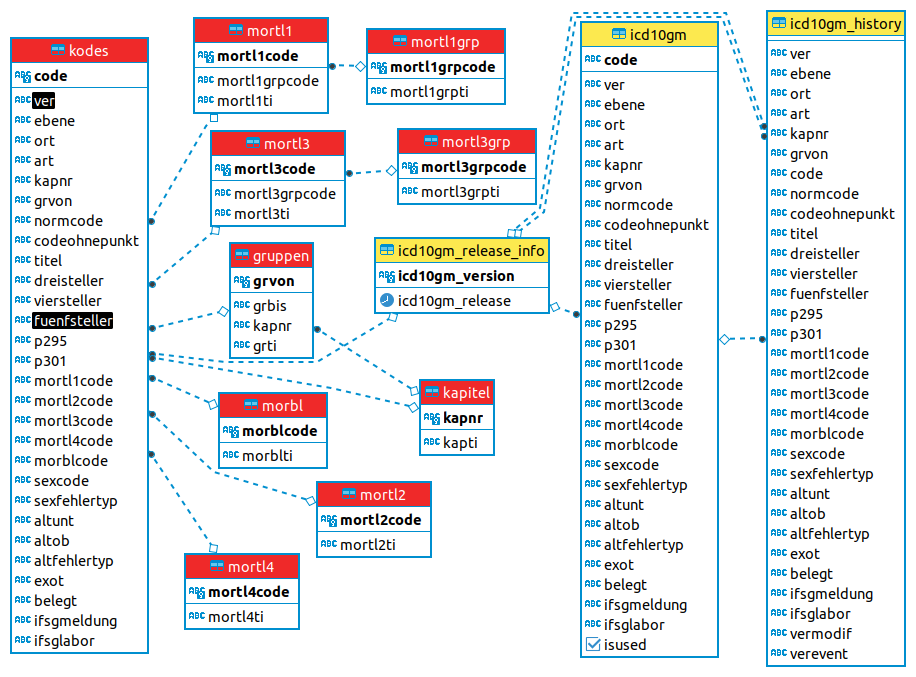
\includegraphics[height=10cm]{figures/icdSqlSchemaNew}
		\caption[Vorschlag der Datenbank Struktur von \acs{icd10gm}]{Datenbank Struktur des Schemas der \ac{icd10gm} von \ac{bfarm} mit der Änderungen an der Tabelle {\ttfamily kodes} in schwarz markiert und neuen Tabellen in gelb gekennzeichnet.}
		\label{fig:reldb2}
	\end{figure}
\subsection{Funktion der neuen Tabellen} \label{newtables}

Für die Erfassung der Datierung der Veröffentlichungen der \ac{icd10gm} wurde die Tabelle {\ttfamily icd10gm\_release\_info} erstellt. Diese speichert den Identifikator oder das Jahr der Version in der Spalte {\ttfamily icd10gm\_version} und das Datum der Veröffentlichung in der Spalte {\ttfamily icd10gm\_release}. Diese hat das Format {\ttfamily JJJJ-MM-TT}. Wobei J das Jahr, M der Monat und T der Tag darstellen.

Die \ac{icd10gm} von 2007 bis 2021, in aktueller Fassung bei den gültigen, werden in der Tabelle {\ttfamily icd10gm} gespeichert. Die Spalte {\ttfamily code}, genau wie bei der Tabelle {\ttfamily kodes} vom \ac{bfarm}-Schema ist die Hauptschlüssel. {\ttfamily ver} speichert die Version und ist ein Fremd Schlüssel, der zeigt die Spalte {\ttfamily icd10gm\_version} der Tabelle {\ttfamily icd10gm\_release\_info}. Die boolesche Spalte {\ttfamily isused} wird benutzt zu markieren welche \ac{icd10gm} bei anderen Systemen angewendet wurde. Die Tabelle {\ttfamily icd10gm} kann auch für Plausibilitätsabfragen benutzt werden.

Die Tabelle {\ttfamily icd10gm\_history} enthält die vorherige Information der \ac{icd10gm}, die mit der Laufe der Zeit gelöscht oder geändert wurden. Die Besonderheiten diese Tabelle sind die Spalten {\ttfamily ver}, {\ttfamily vermodif} und {\ttfamily verevent}. Die Identifikatoren vergangener Versionen einer \ac{icd10gm} werden in der Spalte {\ttfamily ver} gespeichert. Die Spalte {\ttfamily vermodif} enthält der Identifikator der Fassungen bei deren eine \ac{icd10gm} gelöscht oder modifiziert wurde. Die Ereignisse von Änderung oder Löschung werden mit den Buchstaben {\ttfamily U} für \glqq{\ttfamily  update}\grqq{} und {\ttfamily D} für \glqq{\ttfamily  delete}\grqq{} in der Spalte {\ttfamily verevent} kodiert und gespeichert.

\subsection{Fluss der Information} \label{dbrun}

Mit Hilfe einer \ac{etl}-Strecke (Sektion \ref{etlpipeline}) werden die Daten in der \ac{db} importiert. Die Information der Veröffentlichung der \ac{icd10gm} wird in der Tabelle {\ttfamily icd10gm\_release \_info} eingefügt. Die Tabellen von \ac{bfarm} erhalten nur die Information der, für ein Jahr, gültigen \ac{icd10gm}. Mit jeder Ladung wird die Information der Tabelle {\ttfamily icd10gm} mit den Daten der Tabelle {\ttfamily kodes} erneuert. Wobei die neuen Codes und deren Informationen zusammen mit Aktualisierungen eingefügt werden. An diese Stelle die \ac{icd10gm}, die in der neuen Fassung nicht mehr vorhanden sind oder modifiziert wurden, werden in der alten Fassung in der Tabelle {\ttfamily icd10gm\_history} mit der Art der Änderung zusammen mit Identifikator vergangener und neuer \ac{icd10gm} Version eingefügt. Dieser Prozessablauf in der \ac{db} ist durch Triggers gesteuert. Den Fluss der Information ist im Datenflussdiagramm der Abbildung \ref{fig:dbflow} repräsentiert.

\begin{figure}[ht]
	\centering
	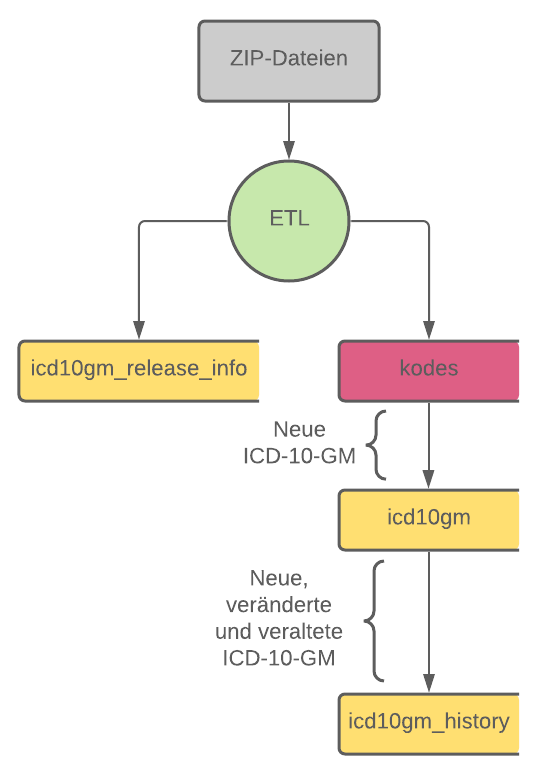
\includegraphics[height=10cm]{figures/dbflow}
	\caption[Datenfluss des Prozesses]{Datenflussdiagramm der Information von den \ac{zip}-Dateien bis zum Import in der \ac{db}}
	\label{fig:dbflow}
\end{figure} 